% Name           : beamerthemeinfurl.sty
% Author         : Victor Orozco (vlorozco@correo.url.edu.gt)
% Version        : 0.1
% Created on     : 13.01.2016
% Last Edited on : 13.01.2016
% Copyright      : Copyright (c) 2016 by Victor Orozco. All rights reserved.
% License        : This file may be distributed and/or modified under the
%                  GNU Public License.
% Description    : Beamer theme using URL logo and colors
%                   based on Benjamin Weiss template, available at 
%                   https://github.com/hsrmbeamertheme/hsrmbeamertheme

\documentclass{beamer}

\usepackage{tikz}
\usepackage[english]{babel}
\usepackage[T1]{fontenc}

\usepackage{smartdiagram}
\usepackage{qtree}
\usepackage{listings}
\lstset{language=Java,
	basicstyle=\footnotesize\ttfamily,
	keywordstyle=\footnotesize\color{blue}\ttfamily,
}

\usetheme{infurl}

\title{Pensamiento sistémico}
\subtitle{Interciclo 2016}
\date{Ultima actualización: \today}
\author{Víctor Orozco}
\institute{{\Medium Ingeniería} URL}

\begin{document}

\maketitle

\section*{TOC}
\begin{frame}
	\frametitle{TOC}
	\tableofcontents[hideallsubsections]
\end{frame}

\section{Introducción}
\begin{frame}
	¿Porque es importante conocer las leyes? 

	\pause
	¿Cual es la ley que hace oficial la existencia de la URL?
\end{frame}

\begin{frame}
		\begin{figure}
			\centering
			
\includegraphics[width=0.9\linewidth]{img/ceps}	
		\end{figure}
\end{frame}

\section{Sistemas}
\begin{frame}{Sistema}
	¿Que hacer para comprender un sistema?
\end{frame}

\begin{frame}{Sistema}
	\begin{enumerate}
		\item Aislarlo 
		\item Simplificarlo
		\item Encontrar sus elementos
	\end{enumerate}
	\pause
	\textbf{Reduccionismo}
\end{frame}


\begin{frame}{Sistema vs pila}
	\begin{enumerate}
		\item Vaca vs. leche
		\item ¿Que obtenemos al sumar varias vacas y varios recipientes de leche?
		\item ¿Que obtenemos al dividir una vaca en partes y un galón de leche en partes?
	\end{enumerate}
\end{frame}

\begin{frame}{Sistema vs pila}
	\begin{figure}
		\centering
		\includegraphics[width=0.9\linewidth]{img/cortes}	
	\end{figure}
\end{frame}

\section{Holismo}
\begin{frame}{Sistema}
	\begin{block}{Definición}
	Conjunto de \textbf{elementos} que se encuentran \textbf{interrelacionados} trabajando en conjunto para alcanzar uno o varios \textbf{objetivos} en común
	\end{block}
\end{frame}

\begin{frame}{Pensamiento sistémico}
	\begin{enumerate}
		\item ¿Que pasa si uno de los elementos cambia?
		\item ¿Que pasa si uno de los elementos desaparece?
		\item ¿Que pasa si uno de los elementos evoluciona?
	\end{enumerate}
\end{frame}

\begin{frame}{Pensamiento sistémico}
	\begin{quote}
"Algunas personas solo ven el árbol y se pierden el bosque a su alrededor"
	\end{quote}

-Anónimo-
\end{frame}


\begin{frame}{Pensamiento sistémico}
	\begin{enumerate}
		\item ¿Empresa?
		\item ¿Vida?
		\item ¿Sociedad?
	\end{enumerate}
\end{frame}

\begin{frame}{Pensamiento sistémico}
	\begin{itemize}
		\item Cambio, adaptación, rebelión
		\item Comprender el mundo como un todo
		\item Enfoque para realizarlo
	\end{itemize}
\end{frame}

\begin{frame}{Pensamiento sistémico}
	\begin{figure}
		\centering
		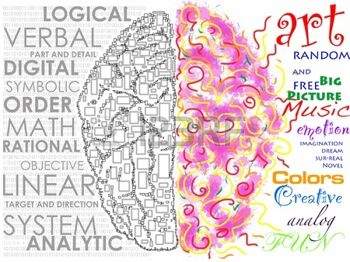
\includegraphics[width=0.7\linewidth]{img/cerebro}	
	\end{figure}
\end{frame}


\begin{frame}{Pensamiento sistémico}
	\begin{enumerate}
		\item Nuevos temas y conocimiento
		\item Problemas complejos
		\item Estrategias efectivas
		\item Visión global
	\end{enumerate}
\end{frame}

\begin{frame}{Pensamiento sistémico}
	\begin{figure}
		\centering
		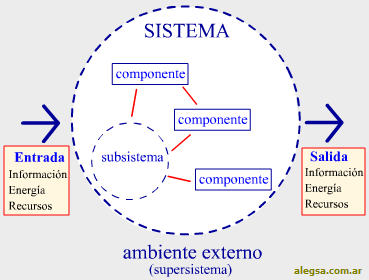
\includegraphics[width=0.9\linewidth]{img/sistema}	
	\end{figure}
\end{frame}

\begin{frame}{Pensamiento sistémico}
	
{\large 	$ \Sigma = C + R + E$}

Componentes

Relaciones (Interrelaciones)

Entorno

\end{frame}

\begin{frame}{Pensamiento sistémico}
	\begin{alertblock}{Definición}
		"Actitud del ser humano para percibir \textbf{el mundo real en términos de totalidades} para su análisis, comprensión y accionar, a diferencia del reduccionismo que solo percibe partes inconexas.
	\end{alertblock}
\end{frame}

\begin{frame}{Pensamiento sistémico}
¿Si los distintos componentes de un sistema actúan juntos como una unidad única, por qué no puede ese sistema ser parte de otro sistema mayor?

\pause
Seguramente sera parte de un sistema mayor
\end{frame}

\begin{frame}{Principios pensamiento sistémico}
	\begin{enumerate}
		\item Equilibro entre corto y largo plazo
		\item Conservar el dinamismo, complejidad e independencia de los sistemas
		\item Tomar en cuenta aspectos cualitativos y cuantitativos
		\item Diversidad de puntos de vista
		\item Considerar siempre la influencia desde y hacia
	\end{enumerate}
\end{frame}

\section{Ejemplos}

\begin{frame}{Alumno - Reduccionismo}
	\begin{quote}
	Mi responsabilidad como alumno es aprender ciencias básicas, aplicadas y complementarias para ser un buen ingeniero".
	\end{quote}
\end{frame}

\begin{frame}{Alumno - Pensamiento sistémico}
	
	\begin{columns}
		\begin{column}{0.5\textwidth}
				"Mi responsabilidad como alumno es desarrollar mis conocimientos, habilidades actitudes y valores para servir a la sociedad de forma sostenible mediante mi actuación como ingeniero, empresario y/o emprendedor".
		\end{column}
		\begin{column}{0.5\textwidth}  %%<--- here
		\begin{figure}
			\centering
			
\includegraphics[width=0.9\linewidth]{img/yoda}	
		\end{figure}
		\end{column}
	\end{columns}
\end{frame}

\begin{frame}{Buenos profesores - Reduccionismo}
		\begin{quote}
	"La universidad debe tener buenos profesores para que los alumnos realmente puedan ser un buen recurso humano en las ciencias y artes para su actuar científico y profesional".
\end{quote}
\end{frame}

\begin{frame}{Profesor - Pensamiento sistémico}
	
	\begin{columns}
		\begin{column}{0.5\textwidth}
			"Los profesores con calidad y exigencia, generan universidades de excelencia que a su vez generan profesionales, empresas y organizaciones competitivas para la creación de una sociedad competitiva a nivel mundial".
		\end{column}
		\begin{column}{0.5\textwidth}  %%<--- here
			\begin{figure}
				\centering
				
\includegraphics[width=0.9\linewidth]{img/proudmeme}	
			\end{figure}
		\end{column}
	\end{columns}
\end{frame}

\begin{frame}{Gracias}
	\begin{center}
		
\includegraphics[width=0.1\linewidth]{img/cclogo}
		\\
		This work is licensed under a Creative Commons Attribution-ShareAlike 3.0 Guatemala License.
	\end{center}
\end{frame}

\end{document}




